%%%%%%%%%%%%%%%%%%%%%%%%%%%%%%%%%%%%%%%%%
% Beamer Presentation
% LaTeX Template
% Version 1.0 (10/11/12)
%
% This template has been downloaded from:
% http://www.LaTeXTemplates.com
%
% License:
% CC BY-NC-SA 3.0 (http://creativecommons.org/licenses/by-nc-sa/3.0/)
%
%%%%%%%%%%%%%%%%%%%%%%%%%%%%%%%%%%%%%%%%%

%----------------------------------------------------------------------------------------
%	PACKAGES AND THEMES
%----------------------------------------------------------------------------------------

\documentclass{beamer}

%\mode<presentation> {
\usetheme{Madrid}

%\setbeamertemplate{footline} % To remove the footer line in all slides uncomment this line
%\setbeamertemplate{footline}[page number] % To replace the footer line in all slides with a simple slide count uncomment this line
%\setbeamertemplate{navigation symbols}{} % To remove the navigation symbols from the bottom of all slides uncomment this line
%}

\usepackage{graphicx} % Allows including images
\usepackage{booktabs} % Allows the use of \toprule, \midrule and \bottomrule in tables

%----------------------------------------------------------------------------------------
%	TITLE PAGE
%----------------------------------------------------------------------------------------

\title[Hubness]{Density and Hubness} % The short title appears at the bottom of every slide, the full title is only on the title page

\author{Libby Beer (libby.beer@gmail.com)\\
Jesse Metcalf-Burton (datasciencejess@gmail.com)\\
Marilyn Vazquez ()} % Your name
\date{\today} % Date, can be changed to a custom date

\begin{document}

\begin{frame}
\titlepage % Print the title page as the first slide
\end{frame}

%\begin{frame}
%\frametitle{Overview} % Table of contents slide, comment this block out to remove it
%\tableofcontents % Throughout your presentation, if you choose to use \section{} and \subsection{} commands, these will automatically be printed on this slide as an overview of your presentation
%\end{frame}

%----------------------------------------------------------------------------------------
%	PRESENTATION SLIDES
%----------------------------------------------------------------------------------------

%------------------------------------------------
%\section{First Section} % Sections can be created in order to organize your presentation into discrete blocks, all sections and subsections are automatically printed in the table of contents as an overview of the talk
%------------------------------------------------

%\subsection{Subsection Example} % A subsection can be created just before a set of slides with a common theme to further break down your presentation into chunks



\begin{frame}
\frametitle{Libby goes here}

\end{frame}

%------------------------------------------------

\begin{frame}
\frametitle{Distances between points? Hubs?}

Can hubs help us cluster?
%\begin{itemize}
%\item Idea to use hubs as initial centers for k-means
%\item ``Outliers'' always mess things up
%\item What happens if we cluster hubs?
%\end{itemize}

\centering
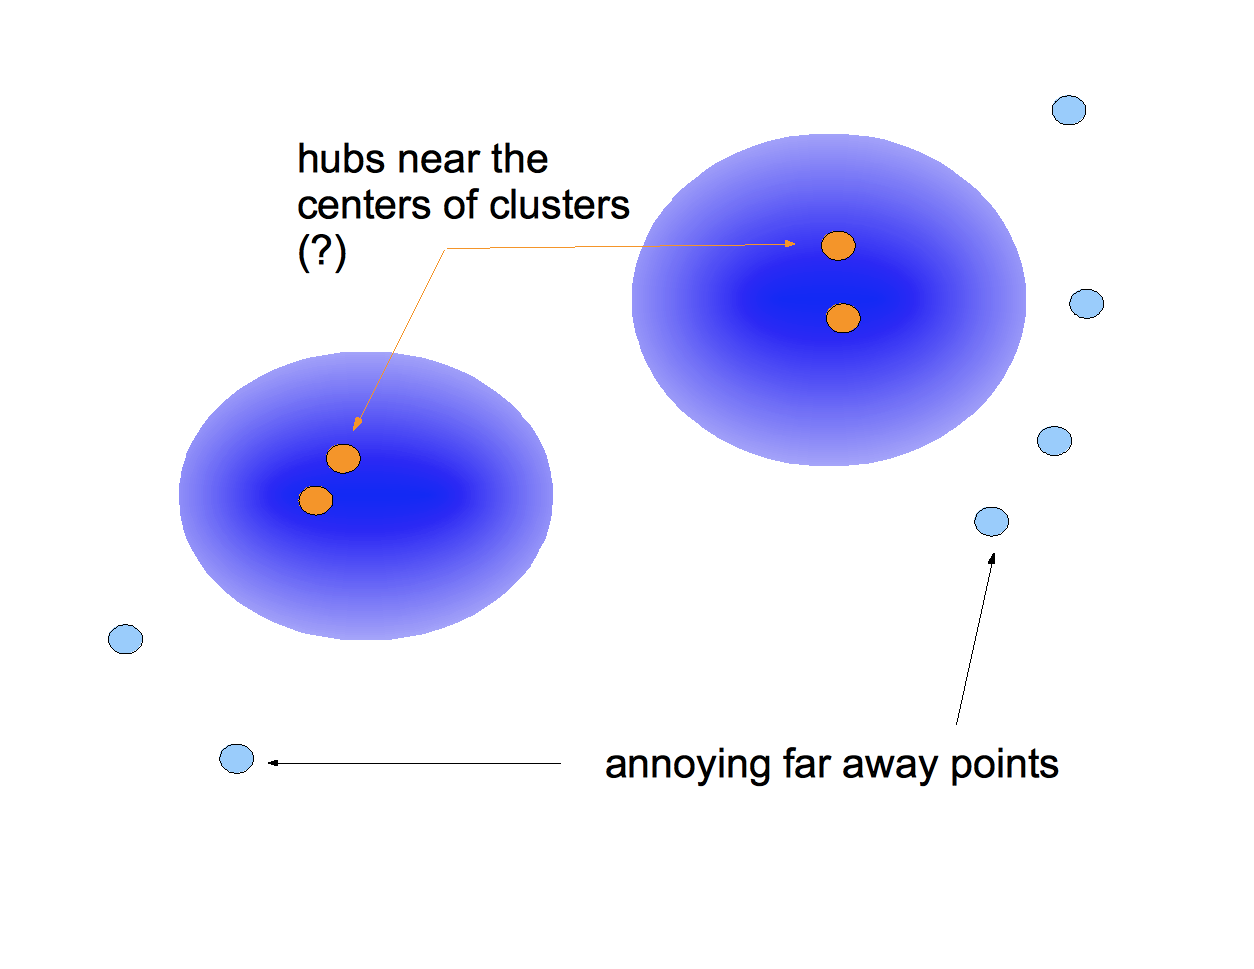
\includegraphics[width=.9\textwidth]{fig/hubness_sketch.png}



\end{frame}

\begin{frame}
\frametitle{Distances with synthetic data}
\centering
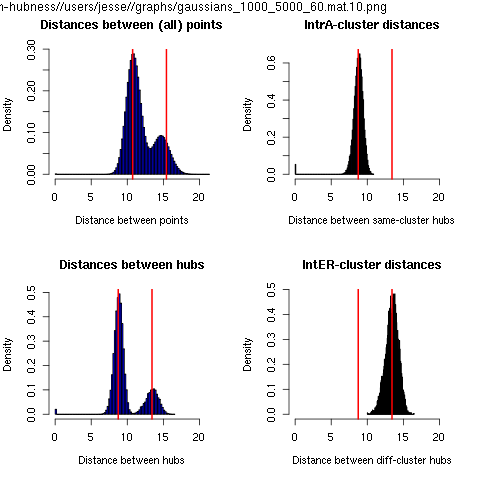
\includegraphics[width=.7\textwidth]{{fig/gaussians_1000_5000_60.mat.10}.png}
%              class0 class1
%   points       1000   3000
%   hubs          33     211 
%  %hubs/class     
\end{frame}

\begin{frame}
\frametitle{Distances with (other) synthetic data}
\centering
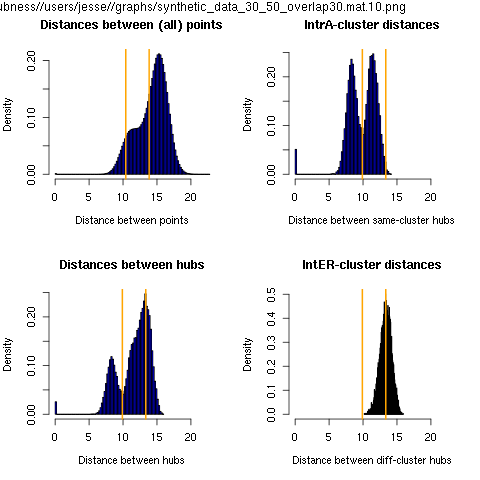
\includegraphics[width=.7\textwidth]{{fig/synthetic_data_30_50_overlap30.mat.10}.png}
%              class0 class1
%   points       2500   2500
%   hubs           93    102
%  %hubs/class     48     52
\end{frame}

\begin{frame}
\frametitle{Distances with real data}
\centering
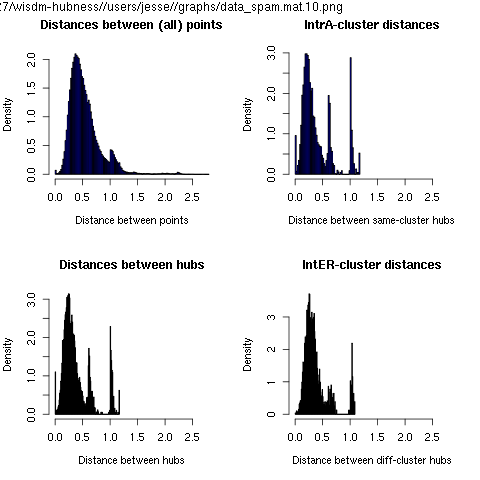
\includegraphics[width=.7\textwidth]{{fig/data_spam.mat.10}.png}
%              class0 class1
%   points       2788   1813
%   hubs          141     55
%  %hubs/class     72     28
\end{frame}


\begin{frame}
\frametitle{Marilyn goes here}

\end{frame}

%------------------------------------------------

\end{document}
